\subsection{Bitvectors} % Inizia la sottosezione

% --- SLIDE 5: Bitvectors and Fundamental Queries ---
\begin{frame}{Bitvectors and Fundamental Queries}
    \framesubtitle{The Simplest Sequence}
    Consider the most basic sequence: a \textbf{bitvector} $B[1..n]$, a sequence of $n$ bits from $\{0, 1\}$.
    \begin{itemize}[<2->]
        \item \textbf{\textsf{rank}}$_b(B, i)$: How many bits $b$ are in the prefix $B[1..i]$? (Count)
        \item \textbf{\textsf{select}}$_b(B, j)$: What is the position (index) of the $j$-th occurrence of bit $b$? (Locate)
    \end{itemize}

    \begin{figure}[htbp]
        \centering
        \only<1-2>{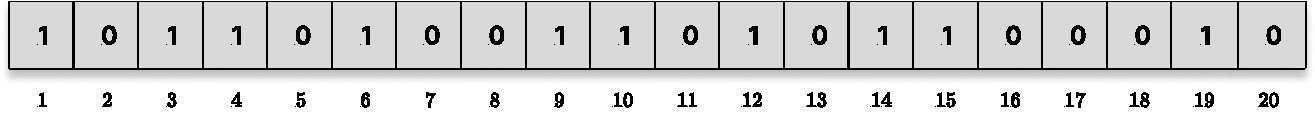
\includegraphics[width=0.9\textwidth]{assets/rank_select_1.pdf}}
        \only<3>{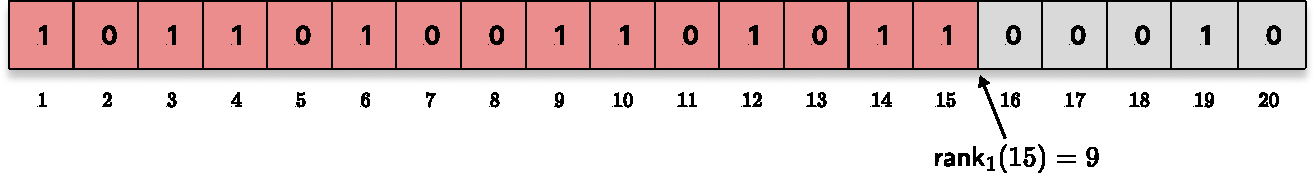
\includegraphics[width=0.9\textwidth]{assets/rank_select_2.pdf}}
        \only<4->{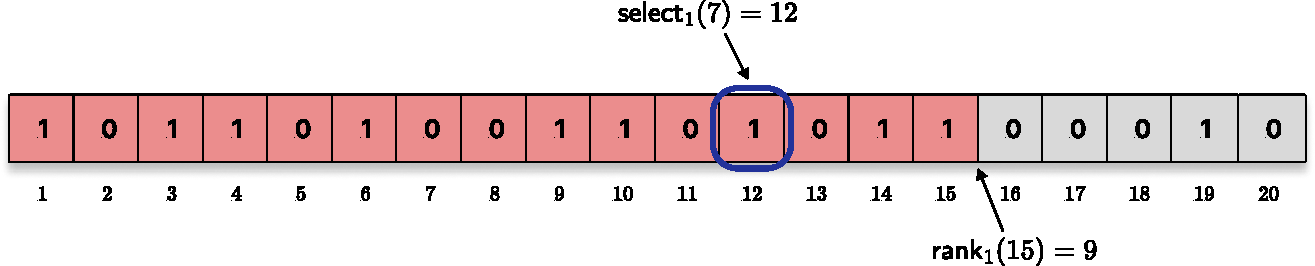
\includegraphics[width=0.9\textwidth]{assets/rank_select_3.pdf}}
    \end{figure}
    \uncover<4->{Furthermore, \textsf{rank} and \textsf{select} are inverse operations:
        \[
            \textsf{rank}_b\bigl(B,\textsf{select}_b(B,j)\bigr)
            = j
            \quad\text{and}\quad
            \textsf{select}_b\bigl(B,\textsf{rank}_b(B,i)\bigr)
            = i.
        \]
    }

\end{frame}

% --- SLIDE 6: RRR Structure: Entropy-Compressed Bitvectors ---
\begin{frame}{RRR Structure: Entropy-Compressed Bitvectors}
    \framesubtitle{Achieving Space Close to Empirical Entropy}
    \begin{block}{Succinct Data Structure for Bitvectors}
        \begin{itemize}
            \item \textbf{Goal:} Support $\textsf{rank}$ and $\textsf{select}$ in $O(1)$ time.
            \item \textbf{Space:} Close to the information-theoretic minimum for the bitvector.
        \end{itemize}
    \end{block}
    \pause

    \begin{theorem}[RRR Structure]
        A bitvector $B[1..n]$ with $m$ set bits can be represented using
        \[ B(n, m) + o(n) + O(\log \log n) \quad \text{bits}, \]
        where $B(n, m) = \lceil \log_2 \binom{n}{m} \rceil$, while supporting \textsf{rank} and \textsf{select} queries in $O(1)$ time.
    \end{theorem}
    $B(n,m) \approx n \mathcal{H}_0(B)$ is the \textbf{information-theoretic minimum space} required to store an arbitrary subset of size $m$ from a universe of size $n$

\end{frame}

% \begin{frame}{\textsf{Rank} on Bitvectors: Succinct $O(1)$ Solution}
%     \framesubtitle{Hierarchical Approach}

%     % Testo con overlay
%     \uncover<1->{How to answer $\textsf{rank}_b(B, i)$ in $O(1)$ time without scanning? $\rightarrow$ Precompute ranks.}
%     \uncover<2->{
%         \begin{itemize}
%             \item<2-> Divide $B$ into \emph{superblocks} (size $Z$). Store absolute ranks ($R_S$).
%             \item<3-> Divide $B$ into \emph{blocks} (size $z$). Store relative ranks ($R_B$).
%             \item<4-> Use a \emph{lookup table} $T$ (or popcount) for ranks within small blocks $z$.
%         \end{itemize}
%     }

%     \begin{figure}[hbtp]
%         \centering
%         % Replace TikZ with sequential images
%         \only<2>{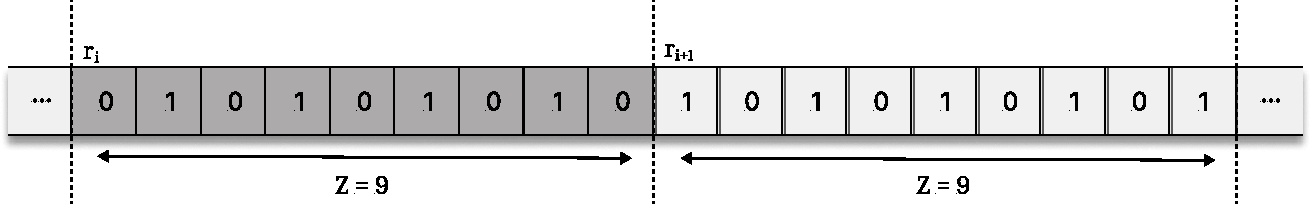
\includegraphics[width=0.7\textwidth]{../bachelor-thesis/TeX/assets/rank1.pdf}} % Visible only on slide 2
%         \only<3>{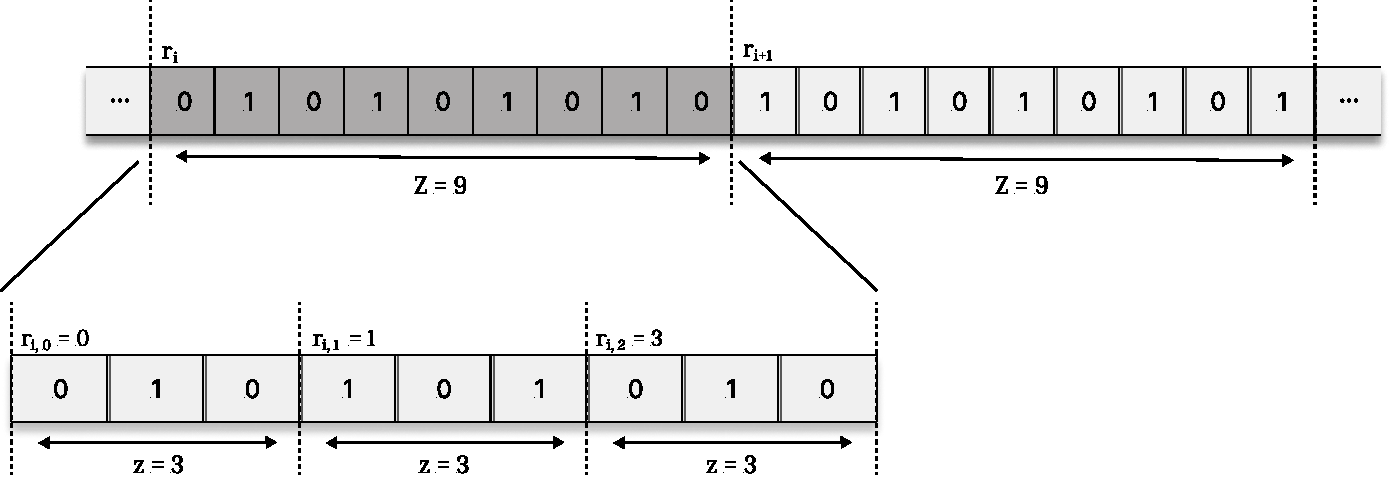
\includegraphics[width=0.7\textwidth]{../bachelor-thesis/TeX/assets/rank2.pdf}} % Visible only on slide 3
%         \only<4->{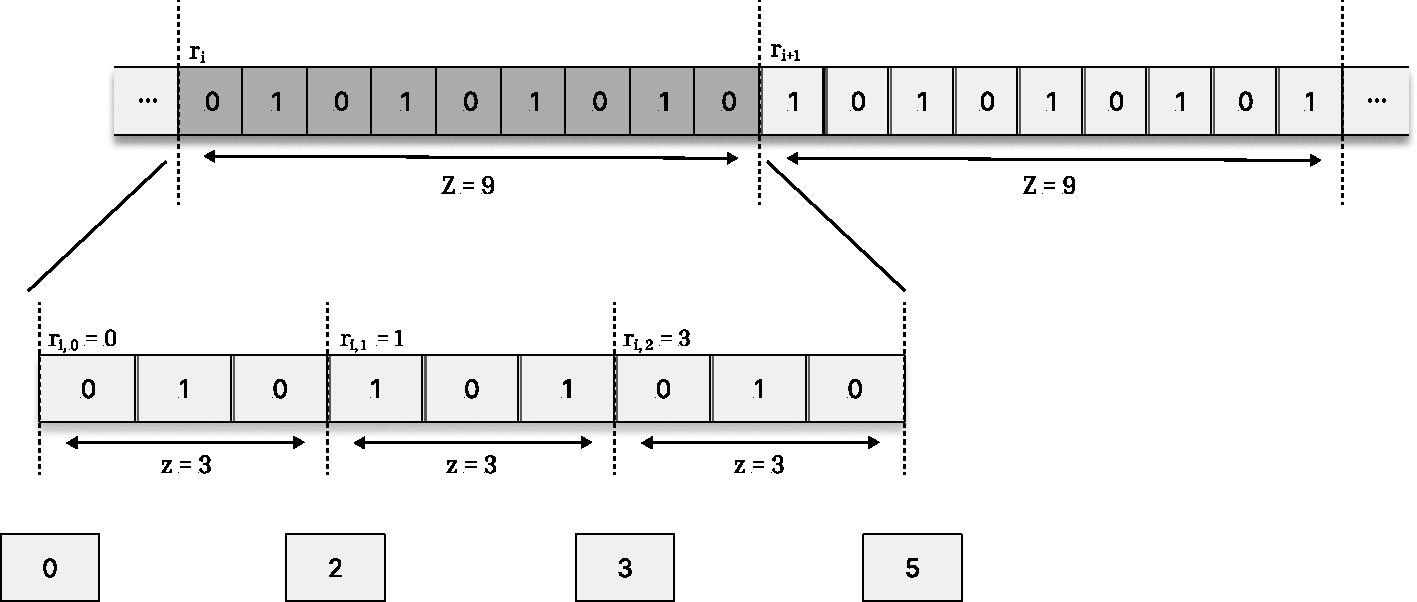
\includegraphics[width=0.7\textwidth]{../bachelor-thesis/TeX/assets/rank3.pdf}} % Visible from slide 4 onwards
%         % Optional caption if needed
%         % \caption{Hierarchical structure for Rank}
%     \end{figure}

% \end{frame}

% \begin{frame}{\textsf{Rank} on Bitvectors: Formal Result}
%     \framesubtitle{Constant Time, Sublinear Space}

%     Building on the hierarchical structure (superblocks, blocks, lookup/popcount):

%     % \bigskip

%     \begin{theorem}<1->[Space Complexity]
%         Given a bitvector $B[1..n]$, there exists an auxiliary data structure using $o(n)$ bits that allows computing $\textsf{rank}_b(B, i)$ for any $i \in [1,n]$ and $b \in \{0,1\}$ in $O(1)$ time.
%     \end{theorem}

%     \bigskip

%     \begin{itemize}
%         \item<2-> The auxiliary structure stores precomputed ranks:
%             \begin{itemize}
%                 \item $R_S$ (Superblock Ranks): $O(n / \log n)$ bits
%                 \item $R_B$ (Block Ranks, relative): $O(n \log \log n / \log n)$ bits
%                 \item $T$ (Intra-block Ranks, efficient impl.): $o(n)$ bits
%             \end{itemize}
%         \item<3-> Total auxiliary space is $o(n)$.
%         \item<4-> The \textbf{total space} required (including the original $n$ bits of $B$) is $\mathbf{n + o(n)}$ bits.
%             % \item<5-> Practical note: For small blocks ($z \le 64$), the intra-block rank is often computed directly using fast CPU instructions (\texttt{popcount}).
%     \end{itemize}

% \end{frame}

% \begin{frame}{\textsf{Select} on Bitvectors: Locating the $i$-th Bit}
%     \framesubtitle{Inverse of Rank}

%     % Definizione e relazione con Rank
%     \uncover<1->{
%         The \textbf{\textsf{select}}$_b(B, i)$ operation finds the position $j$ of the $i$-th bit $b$.
%         \[ \textsf{rank}_b(B, \textsf{select}_b(B, i)) = i \]
%         It answers "Where is the $i$-th $b$?".
%     }

%     \bigskip

%     % Approccio e idea chiave (Clark '97)
%     \uncover<2->{
%         Achieving $O(1)$ time requires a different auxiliary structure than \textsf{rank}
%         \begin{itemize}
%             \item Core Idea: Hierarchy based on the \textbf{cumulative count of 1s}, not fixed positions.
%             \item Strategy: Use multiple levels of indexing to quickly narrow down the region in $B$ containing the $i$-th 1.
%         \end{itemize}
%     }

% \end{frame}

% \begin{frame}{\textsf{Select} on Bitvectors: Hierarchical Structure}
%     \framesubtitle{Handling Sparsity}

%     % Struttura Gerarchica (semplificata)
%     \uncover<1->{
%         Multi-level Structure Overview (Clark '97):
%         \begin{itemize}
%             \item<1-> Level 1: Divide $B$ into variable-length \emph{chunks}, each containing exactly $K$ ones. Store chunk start positions ($P_1$). $\rightarrow$ Quickly locate the chunk of the $i$-th 1.
%             \item<2-> Differentiate chunk handling based on density (length vs $K$):
%                 \begin{itemize}
%                     \item \emph{Sparse} chunks (long): Store relative positions of the $K$ ones directly. $O(1)$ lookup.
%                     \item \emph{Dense} chunks (short): Need further subdivision.
%                 \end{itemize}
%             \item<3-> Level 2 (for dense chunks): Subdivide into \emph{sub-chunks} with $k$ ones. Store relative sub-chunk starts ($P_2$). Handle sparse/dense sub-chunks recursively or with a base-case mechanism (lookup/popcount for very dense).
%         \end{itemize}
%     }

%     % Risultato finale
%     \uncover<4->{
%         \begin{theorem}
%             This multi-level structure uses $o(n)$ auxiliary bits and supports $\textsf{select}_b(B, i)$ in $O(1)$ time.
%             Total space remains $\mathbf{n + o(n)}$ bits.
%         \end{theorem}
%     }
% \end{frame}
